\documentclass{beamer}
\usepackage{../preamble/custom}

\setbeamertemplate{bibliography item}[text]

\title{Maximal repetition \& ``Runs'' conjecture}
\author{Riccardo Lo Iacono \\ \footnotesize{Docente: Gabriele Fici}}
\begin{document}
    \begin{frame}
        \maketitle
    \end{frame}
    \begin{frame}{Notazione}
        \begin{enumerate}
            \item \(\Sigma\) è un alfabeto ordinato e finito di simboli
            \item Un elemento \(S \in \Sigma^{*}\) è detto stringa,
                la cui lunghezza è denotata da \(\abs{S}\)
            \item Per ogni i, \(1 \le i \le n = \abs{S}\), 
                S[i] indica l'i-esimo carattere in S.
            \item Per ogni i, j, \(1 \le i \le j \le n = \abs{S}\),
                S[i, j] indica la sottostringa compresa tra le 
                posizioni i e j, 
        \end{enumerate}
    \end{frame}
    \begin{frame}{Periodo ed esponente}
        \textbf{Definizione: } Data S una stringa,
        si definisce \emph{periodo} un intero \(p \ge 1\)
        tale che S[i] = S[i + p], \(\forall i = 1, \ldots, \abs{S} - p\)

        \textbf{Definizione: } Si definisce \emph{esponente} \(\exp\)
        il rapporto tra la lunghezza di S e del suo più piccolo periodo.
    \end{frame}
    \begin{frame}{Ripetizioni massimali}
        \textbf{Definizione: } Una coppia (i, j) è detta ripetizione massimale
        (o run) di una stringa S, se \(\exp(S[i, j]) \ge 2\) e la periodicità
        non può essere estesa nè a destra ne a sinistra.
    \end{frame}
    \begin{frame}{Un esempio}
        Sia considerata la stringa \(S = babbabbababbabbabc\); questa contiene nove 
        run, mostrati in \emph{Figura \ref{fig:1}}.

        \begin{figure}[!h]
            \centering
            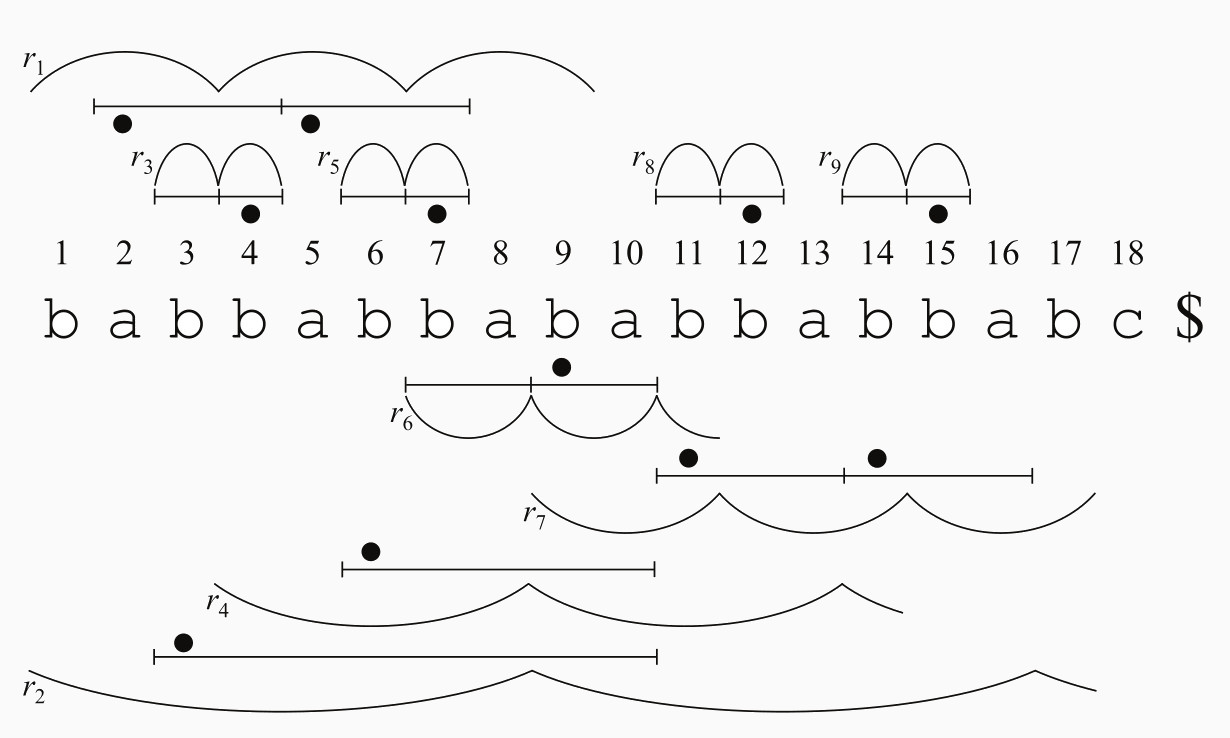
\includegraphics[scale = .85]{../Extra/run example.jpg}
            \caption{Illustrazione dei run nella stringa S = babbabbababbabbabc.}
            \label{fig:1}
        \end{figure}
    \end{frame}
    \begin{frame}{Background storico}
        Sia \(\rho(S)\) il numero dei run in una stringa S.

        \emph{Kolpakov \emph{e} Kucherov}\footnotemark[1]
        dimostrano che \(\rho(S) = \bigO{|S|}\).
        \vskip 10pt
        \textbf{Congettura (Runs conjecture):} \(\rho (S) < |S|\) per ogni stringa S.

        \footnotetext[1]{R. M. KUCHEROV {\footnotesize AND} G. KOLPAKOV,
            \emph{Finding maximal repetitions in a word in linear time. FOCS, 1999}
        }
    \end{frame}
    \begin{frame}{Premessa}
        Si puntualizza che la congettura è stata dimostrata per la prima 
        volta da Bannai et al.\footnotemark[2]
        
        La dimostrazione di Bannai et al. risulta essere complessa,
        per tale ragione sarà analizzata la versione proposta da Crochemore e Mercas.\footnotemark[3]

        \footnotetext[2]{HIDEO BANNAI, TOMOHIRO I, SHUNSUKE INENAGA,
            YUTO NAKASHIMA, MASAYUKI TAKEDA \footnotesize{AND} KAZUYA TSURATA, 
            \emph{The ``Runs'' Theorem. SODA, 2015}
        }

        \footnotetext[3]{MAXIME CROCHEMORE \footnotesize{AND} ROBERT MERCAS,
            \emph{On density of Lyndor roots in factors. Theorical computer science, 2016}
        }
    \end{frame}
    \begin{frame}{Lyndon words}
        Data S una stringa e i un indice, con \(1 \le i \le n\),
        la stringa S[i,n]S[1,i - 1] è detta \emph{shift ciclico} di S 
        (se i > 1 \emph{shift ciclico non banale}).

        \textbf{Definizione (Lyndon word): } Fissato un certo ordine, 
        una stringa \(S \in \Sigma^{*}, S \ne \varepsilon\),
        è detta Lyndon word se S è minore di ogni suo shift ciclico non banale.
    \end{frame}
    \begin{frame}        
        Assunto \(\prec_{0} \text{ ordine totale su } \Sigma\), 
        si può definire \(\prec_{1}\) l'ordine rovesciato. 
        Ossia, un'ordine tale per cui presi \(a, b \in \Sigma\), se 
        \[
            a \prec_{0} b \implies b \prec_{1} a
        \]
    \end{frame}
    \begin{frame}{La ``Runs'' conjecture}
        \textbf{Teorema: } \(\rho(S) < \abs{S}\), per ogni stringa S.

        \textbf{Dimostrazione: } Sia S una stringa di lunghezza n,
        e sia (i, j), \(1 \le i < j \le n\), un run di periodo minimo p in S.

        Se j + 1 < n, ed inoltre S[j - p + 1] \(\prec_{0}\) S[j + 1],
        si assegna al run un indice k per cui S[k, j] è il \emph{greatest proper suffix}
        di S[i, j]. Viceversa k definisce il più grande suffisso per \(\prec_{1}\).

        Si noti che se k > i allora k > 0, e S[k, j] contiene un intero periodo del run.
        Inoltre, S[k, k + p - 1] è il più grande coniugato di S[i ,i + p - 1]
        rispetto uno dei due ordini. 
        Pertanto è \emph{border-free}, che è una proprietà nota delle Lyndon word.
    \end{frame}
    \begin{frame}
        Si intende dunque dimostrare che ogni k > 0 è posizione iniziale 
        di al più un solo \emph{greatest proper suffix} in un run.

        Siano quindi considerati due run: (i, j) e (l, m) rispettivamente
        un p-run e un q-run. Inoltre, sia assunto per assurdo che 
        i loro greatest proper suffix condividano la stessa posizione iniziale k.

        Sia assunto \(p \ne q\) poichè i run non possono essere distinti è avere lo stesso periodo.
    \end{frame}
    \begin{frame}
        \begin{enumerate}
            \item Sia j = l, ma allora S[k, j] = S[k, m].
                Assumendo per esempio p < q. Allora, S[k, k + q - 1] ha periodo p,
                e quindi questa non è border-free, che è una contraddizione.

            \item Sia asunto sensa perdita di generalità che j < m, 
                e che i suffissi siano i più grandi rispetto un stesso ordine nei rispettivi run, sia questi \(\prec_{0}\).
                Sia d = S[j + 1], il carattere successivo il p-run.
                
                Per definizione si ha che S[j - p + 1] \(\prec\) d e di conseguenza S[k, k - p + 1] \(\prec\) S[k, j - p]d. 
                Ma poichè S[i + p, j] è fattore del q-run, ciò contraddice la massimalita di S[k, m - 1].
        \end{enumerate}
    \end{frame}
    \begin{frame}
        \begin{enumerate}
            \item [3.] Sia \(j \ne m\) e i suffissi risultano i più grandi secondo ordini diversi.
                Senza perdita di generalità sia p < q e il suffisso del p-run
                sia il più grande rispetto \(\prec_{0}\).
                Poichè q > 1, si ha sia che S[k + q - 1] \(\prec_{0}\) S[k] sia che 
                S[k + q - 1] = S[k  - 1], da cui S[k - 1] \(\prec_{0}\) S[k].
                
                Si ha però che p \(\not>\) 1, viceversa si avrebbe S[k] \(\prec_{0}\) S[k - 1]. 
                Inoltre, p \(\ne\) 1 poichè si avrebbe che S[k - 1] = S[k]. 
                Da cui un'altra contraddizione.
        \end{enumerate}

        Ciò conclude la dimostrazione, 
        mostrando come il numero di run non possa essere superiore agli n - 1 
        potenziali valori di k, come supposto.
    \end{frame}
\end{document}
